\chapter{Background and Related Work}
\label{ch:relatedwork}

%%%%%%%%%%%%%%%%%%%%%%%%%%%%%%%%%%%%%%%%%%%%%%%%%%%%%%%%%%%%%%%%%%%%%%%%
\section{The Inverse Problem}
\label{sec:inverse-problem}

Forward models map a set of input parameters to observable outputs. An inverse problem begins with the observations and searches for input or model parameters that are consistent with them. Model calibration performs this inference by comparing simulator outputs with observed data. The inverse relationship is generally not unique. Several parameter combinations may explain the observations equally well, especially in the presence of measurement uncertainty and discrepancies between the simulator and reality \autocite{Kennedy2001,Arendt2012}. Figure~\ref{fig:forward-inverse-problem} illustrates the relationship between the forward and inverse problems.

\begin{figure}[!htbp]
    \centering
    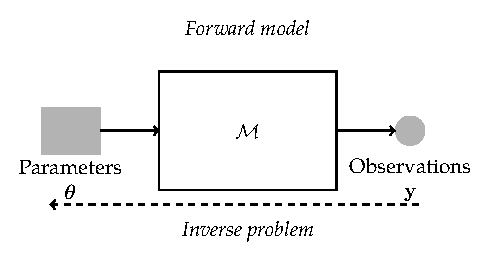
\includegraphics[width=0.8\textwidth]
        {images/forward_inverse_problem.pdf}
    \caption[Relationship between the forward and inverse problems.]
    {Relationship between the forward and inverse problems. The forward model maps parameters $\symbf{\theta}$ to predicted observables, whereas the inverse problem uses observations $\symbf{y}$ to obtain plausible parameter values. Adapted from the conceptual illustration by \textcite{MouraNeto2013}.}
    \label{fig:forward-inverse-problem}
\end{figure}

In inverse-problem theory, a problem is called ill-posed if a solution does not exist, is not unique, or changes strongly under small changes in the data \autocite[Chap.~3]{MouraNeto2013}. Calibration problems often face the latter two issues: because of measurement noise, limited data, and model error, several different parameter combinations can fit the observations equally. Two common solutions are regularization and probabilistic methods, which add extra information about the unknown parameters \autocite{Stuart2010,BenningBurger2018}. This study follows the probabilistic approach. In gravity-driven mass flow modeling, Bayesian calibration is often used, which estimates effective friction parameters from observed events and also quantifies the remaining uncertainty \autocite{Heredia2020,ZhaoKowalski2022}.
 
%%%%%%%%%%%%%%%%%%%%%%%%%%%%%%%%%%%%%%%%%%%%%%%%%%%%%%%%%%%%%%%%%%%%%%%%
\section{The Bayesian Approach to the Inverse Problem}
\label{sec:bayesian-approach}

Bayesian calibration treats the unknown model parameters as uncertain quantities and uses Bayes' theorem to update prior information with observed data. Let $\theta$ denote the model parameters and $y$ the observations. The prior distribution $p(\theta)$ represents information about the parameters before considering $y$, while the likelihood $p(y \mid \theta)$ describes how compatible the observations are with a given parameter value. Bayes' theorem combines these components into the posterior distribution:

\begin{equation}
    p(\theta \mid y)
    =
    \frac{p(y \mid \theta)\,p(\theta)}{p(y)},
    \label{eq:bayes-theorem}
\end{equation}

where $p(y)$ is the model evidence, which does not depend on $\theta$ and normalizes the posterior distribution.

The evidence can be written as $p(y)=\int p(y\mid\theta)p(\theta)\,\mathrm{d}\theta$, but this integral is generally not available to us. Because $p(y)$ is constant with respect to $\theta$, many MCMC methods can explore the posterior using only its unnormalized density \autocite{Kennedy2001,Albert2025}:

\begin{equation}
    p(\theta \mid y)
    \propto
    p(y \mid \theta)\,p(\theta).
    \label{eq:unnormalized-posterior}
\end{equation}

In computation, the unnormalized posterior is commonly evaluated on the logarithmic scale. This converts the product into a sum and reduces numerical errors (in floats) when the probability densities are very small:

\begin{equation}
    \log \widetilde{p}(\theta \mid y)
    =
    \log p(y \mid \theta)
    +
    \log p(\theta),
    \label{eq:log-posterior}
\end{equation}

where $\widetilde{p}(\theta \mid y)$ denotes the unnormalized posterior density. While many MCMC methods require only the unnormalized posterior, nested sampling also estimates the model evidence by rewriting it as a one-dimensional integral of the likelihood over prior mass \autocite{Skilling2006}. In \texttt{dynesty}, this approach is implemented by supplying the likelihood and prior-transformation functions separately \autocite{Speagle2020}.

% Likelihood
The likelihood connects the observations to the output of the forward model. The calibration framework uses an additive Gaussian residual model:

\begin{equation}
    y_i
    =
    f_i(\theta)
    +
    \varepsilon_i,
    \qquad
    \varepsilon_i
    \overset{\mathrm{iid}}{\sim}
    \mathcal{N}(0,\sigma^2),
    \label{eq:additive-error-model}
\end{equation}

where $f_i(\theta)$ denotes the model prediction corresponding to observation $y_i$, and $\sigma$ is the residual standard deviation. Under this assumption, the log-likelihood for $n$ observations is

\begin{equation}
    \log p(y \mid \theta,\sigma)
    =
    -\frac{n}{2}\log(2\pi\sigma^2)
    -
    \frac{1}{2\sigma^2}
    \sum_{i=1}^{n}
    \left(y_i-f_i(\theta)\right)^2.
    \label{eq:gaussian-log-likelihood}
\end{equation}

For the general formulation, $f_i(\theta)$ denotes the full forward-model response. In the benchmark implementation, it is replaced by the surrogate prediction $\widehat{f}_i(\theta)$.

The residual term may combine the model error and measurement error. Consequently, independent Gaussian residuals are assumptions rather than a property guaranteed by the observations \autocite{Kennedy2001,Brynjarsdottir2014,Heredia2020}.

For a Bayesian calibration, each likelihood evaluation generally requires a separate model simulation. For full computational models, this is generally expensive. Therefore, one may utilize a surrogate model that approximates the input-output relationship of the original forward model using a selected set of precomputed runs from an initial training data set \autocite{Gu2024,Yildiz2023}. As a result, the cost of repeated model evaluations is reduced, but the original model response is now replaced by the approximations produced by the surrogate model. Therefore, its accuracy and uncertainty must be considered when interpreting the posterior obtained from these results \autocite{Gu2024,Yildiz2023,ZhaoKowalski2022}.

In this study, instead of using the full gravity-driven mass flow simulator, the likelihood is calculated using the RobustGaSP surrogate. Even though a surrogate evaluation is cheaper than a full model run, it is still performed repeatedly, and different sampling methods may require different numbers of evaluations to reach the desired results.

\section{The Bayesian Calibration Pipeline}
\label{sec:bayesian-calibration-pipeline}

So far, we have seen that Bayesian calibration assigns prior distributions to the unknown parameters, the forward model or surrogate model maps these parameters to predicted observables, and the likelihood compares these predictions with the observed data. These components should be kept separate, since changing the surrogate, prior, likelihood, or observations may lead to a change in the target posterior, whereas changing the sampler only changes the numerical approach used to approximate the target distribution.

Figure~\ref{fig:general-calibration-workflow} provides a broader view of this process, including the construction of a surrogate model from the forward model, as well as the calibration and diagnostic stages.

\begin{figure}[!htbp]
    \centering
    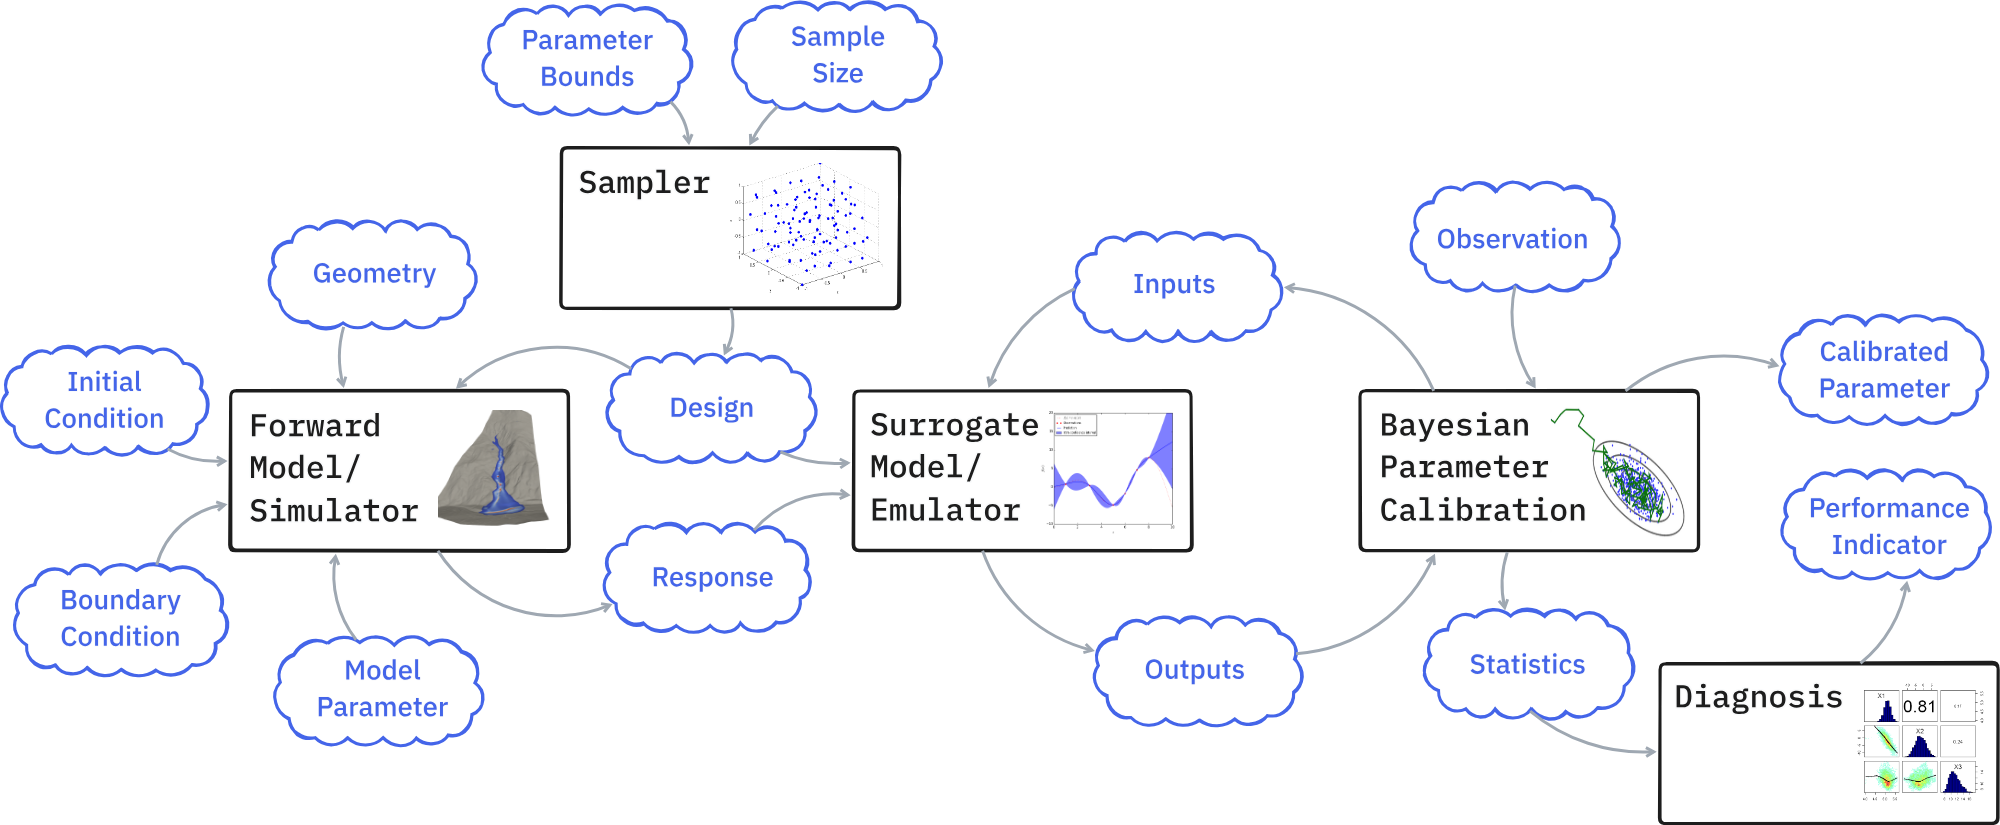
\includegraphics[width=\textwidth]{images/diagram.png}

    \caption[General workflow of Bayesian calibration.]
    {General workflow of Bayesian calibration. Illustration courtesy of Alan Correa.}

    \label{fig:general-calibration-workflow}
\end{figure}

The \texttt{mcmc-bench} framework implements this concept by separating model evaluation from sampler execution. Here, the RobustGaSP surrogate is used through UM-Bridge, so sampler implementations interact with it through a common, language-agnostic interface rather than depending directly on the surrogate's internal implementation \autocite{Gu2024,Yildiz2023,Seelinger2023}. Nextflow coordinates the sampler-specific software environments and the diagnostic and reporting steps within a reproducible computational workflow \autocite{DiTommaso2017}.


\section{Sampling Methods for Bayesian Inference}
\label{sec:sampling-methods}

Modern Bayesian computation includes gradient-based methods such as HMC and NUTS, ensemble and slice-based approaches, population methods such as Sequential Monte Carlo, nested-sampling algorithms, and more recent methods that use normalizing flows to construct proposals or transform the sampling space. Representative implementations use several programming languages and software packages, as summarized in Table~\ref{tab:samplers}.

\begin{table}[htbp]
\centering
\caption{Selected state-of-the-art sampling algorithms.}
\label{tab:samplers}
\begin{tabular}{@{}
  >{\raggedright\arraybackslash}p{0.24\textwidth}
  >{\raggedright\arraybackslash}p{0.16\textwidth}
  >{\raggedright\arraybackslash}p{0.10\textwidth}
  >{\raggedright\arraybackslash}p{0.40\textwidth}@{}}
\toprule
\multicolumn{1}{c}{Algorithm} & \multicolumn{1}{c}{Package(s)} & \multicolumn{1}{c}{Language(s)} & \multicolumn{1}{c}{Benefit(s)} \\
\midrule
HMC/NUTS \autocite{Duane1987,Hoffman2014}
    & PyMC \autocite{PyMCNUTS2026} & Python
    & Gradient-informed exploration \\
Affine-invariant ensemble \autocite{Goodman2010,ForemanMackey2013}
    & emcee & Python
    & Robustness to linear rescaling and correlation \\
Slice sampling \autocite{Neal2003}
    & PyMC \autocite{PyMCSlice2026} & Python
    & Adaptive interval construction \\
SMC \autocite{DelMoral2006}
    & PyMC \autocite{PyMCSMC2026} & Python
    & Population-based exploration \\
Nested sampling \autocite{Skilling2006,Speagle2020,Buchner2021}
    & dynesty, UltraNest & Python
    & Posterior and evidence estimation \\
Flow-based nested sampling \autocite{Williams2021}
    & nessai & Python
    & Learned constrained-prior proposals \\
Flow-enhanced MCMC \autocite{Wong2023}
    & flowMC & Python
    & Learned global proposals for complex posteriors \\
\bottomrule
\end{tabular}
\end{table}

Given the time constraints of the present work, the initial benchmark integrations focus on Python-based packages. This is an implementation-scope decision rather than a limitation of the underlying framework.

This study includes five gradient-free sampling methods. Random-Walk Metropolis-Hastings uses local random-walk proposals with an accept/reject decision \autocite{Hastings1970}. Affine-invariant ensemble sampling uses interacting walkers and reduces sensitivity to linear transformations of the parameter space \autocite{Goodman2010,ForemanMackey2013}. Slice sampling constructs and samples from a region under the probability density around the current state \autocite{Neal2003}. Sequential Monte Carlo evolves a population of weighted particles through a sequence of intermediate distributions \autocite{DelMoral2006}. Nested sampling explores constrained likelihood regions and additionally estimates the model evidence \autocite{Skilling2006,Speagle2020}. These methods have different tuning requirements and computational costs \autocite{Albert2025}.

In the benchmark, these methods are represented by the custom \texttt{rwmcmc} implementation, \texttt{emcee}, the Slice and SMC implementations in PyMC, and \texttt{dynesty}, respectively. Their integration into the common framework is described in Chapter~\ref{ch:ownwork}.
